\documentclass{article}
\usepackage{pshacks}
\usepackage{graphics,amsmath,mathrsfs}
\newcommand{\subscr}[2]{#1_{\textup{#2}}}
\newcommand{\supscr}[2]{#1^{\textup{#2}}}
\newcommand{\supind}[2]{{#1}^{[#2]}}
\newcommand{\network}{\Sigma}
\newcommand{\networkint}{\subscr{\Sigma}{eng}}
\newcommand{\cprice}{\subscr{P}{charge}}
\newcommand{\dprice}{\subscr{P}{discharge}}
\newcommand{\vect}[1]{#1}

 \definecolor{MyBlue}{cmyk}{.5,.7,0,0}
\definecolor{illini}{rgb}{0.98,0.4,0.05}
\definecolor{htmlgreen}{cmyk}{.250,0,1,0.2}
\definecolor{darkgreen}{rgb}{0,0.5,0}
 \definecolor{myblue}{cmyk}{.98,0.10,0,.25}
 \definecolor{myred}{cmyk}{0, .80, .79, 11}
 \definecolor{mygreen}{cmyk}{.50, 0, 1.00, .20}	
 \definecolor{steelblue}{cmyk}{.61, .28, 0, 0}
 \definecolor{darkorange}{cmyk}{0, .50, 1.00, .7}
  \definecolor{oregonsalmon}{cmyk}{0, .53, .87, 0}
    \definecolor{goldgreen}{cmyk}{.39, 0, .39, .07}
       

 
\usepackage[T1]{fontenc}
%\usepackage[T1]{fontenc}
 \usepackage[osf]{mathpazo}

\begin{document}
\small

\begin{psdraw}(-2cm,7cm)(0,0)

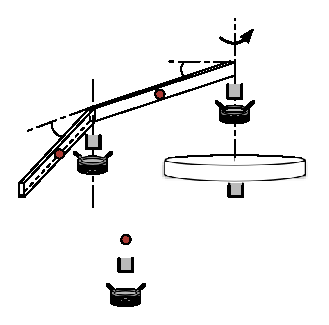
\includegraphics[width=0.7\linewidth]{rotary_flexible_beam_3DOF_breakdown.eps}
\scalelines{0.9}


\move(-1.1,7.8)
\htext{$\tau, \theta > 0$}

\move(-4.3,6.8)
\htext{$\alpha_1 > 0$}

\move(-7.9,4.8)
\htext{$\alpha_2 > 0$}

\move(-1.7,3.5)
\htext{$B_r$}

\move(-1.7,6.2)
\htext{$B_{b_1}$}

\move(-1.5,5.6)
\htext{$K_{b_1}$}

\move(-5.7,4.8)
\htext{$B_{b_2}$}

\move(-5.5,4.2)
\htext{$K_{b_2}$}

\move(-3.9,2)
\htext{$:=$ centre of mass}

\move(-3.7,1.2)
\htext{$:=$ viscous damper}

\move(-3.5,0.3)
\htext{$:=$ torsional spring}

\move(-2.2,3.95)
\htext{rotary servo base}

\end{psdraw}
\end{document}
